\begin{frame}
    \frametitle{CUDA}
    \framesubtitle{Introduction}
    \begin{itemize}
        \item Compute Unified Device Architecture (CUDA).
        \item Computing engine in Nvidia GPUs.
        \item Some advantages:
        \begin{itemize}
            \item Scattered reads.
            \item Shared memory.
            \item Faster communication between CPU/GPU.
            \item etc.
        \end{itemize}
    \end{itemize}
\end{frame}

\begin{frame}
    \frametitle{CUDA}
    \framesubtitle{Program structure}
    \begin{figure}
        \centering
        \label{fig:cuda-structure}
        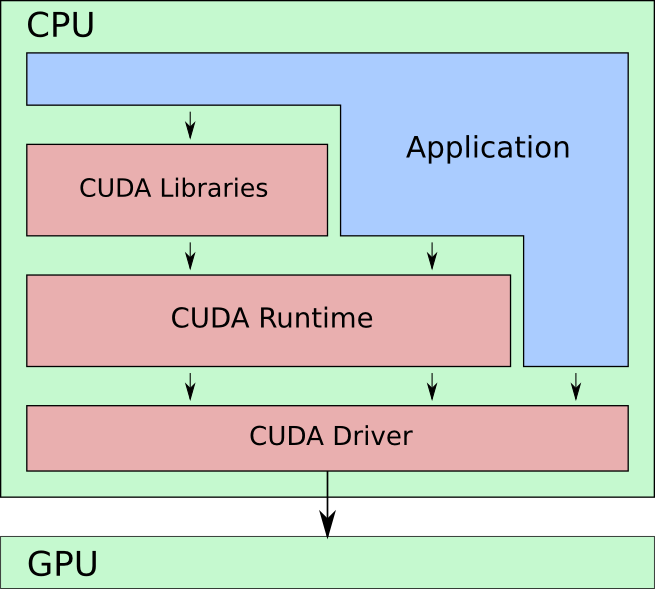
\includegraphics[width=0.5\textwidth]{img/cuda-structure}
        \caption{Program structure}
    \end{figure}
\end{frame}

\begin{frame}[fragile]
    \frametitle{CUDA}
    \framesubtitle{Program structure - Example}
    \begin{lstlisting}
       __global__ void VecAdd(float* A, float* B, float* C)
        {
            int i = threadIdx.x;
            C[i] = A[i] + B[i];
        }

        int main()
        {
            ...
            // Llamada kernel con N hebras en 1 bloque
            VecAdd <<< 1 , N >>> (A, B, C);
            ...
        }
    \end{lstlisting}
\end{frame}



\begin{frame}
    \frametitle{CUDA}
    \framesubtitle{Threads}
    \begin{itemize}
        \item Lighweight.
        \item Efficients.
        \item Cooperation.
        \item Synchronization.
        \item Organization and programming.
    \end{itemize}
\end{frame}

\begin{frame}
    \frametitle{CUDA}
    \framesubtitle{Threads execution model}
    \begin{figure}
        \centering
        \label{fig:cuda-threads}
        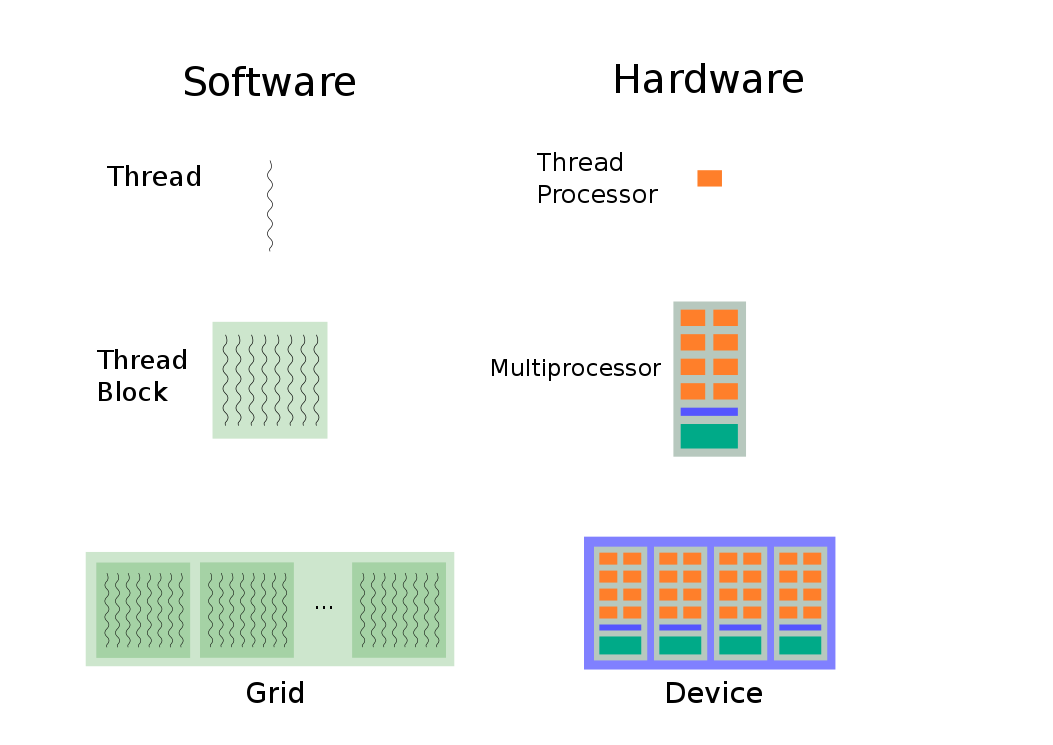
\includegraphics[width=0.5\textwidth]{img/cuda-threads}
        \caption{Threads and blocks on the Hardware and Software}
    \end{figure}
\end{frame}

\begin{frame}
    \frametitle{CUDA}
    \framesubtitle{Memories}
    \begin{figure}
        \centering
        \label{fig:cuda-memories}
        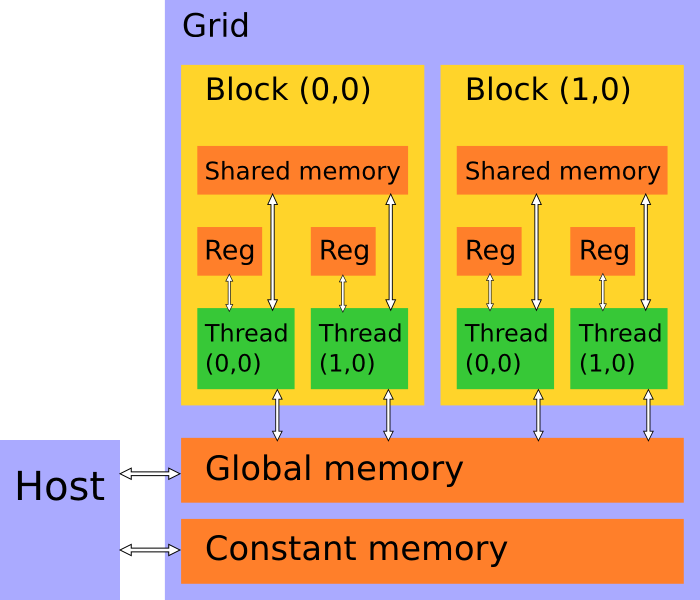
\includegraphics[width=0.5\textwidth]{img/cuda-memories}
        \caption{GPU Memories}
    \end{figure}
\end{frame}

\begin{frame}[fragile]
    \frametitle{CUDA}
    \framesubtitle{Memories}
    \begin{table}
    \centering
    \label{tab:memories-penalty}
    \scriptsize
    \begin{tabular}{l|r|r|r|r}
        \textbf{Declaration}  & \textbf{Memory}   & \textbf{Scope}  & \textbf{Lifetime}    & \textbf{Penalization} \\
        \texttt{int var;}                      & Register & Thread & Thread      & 1x \\
        \texttt{int a\_var[10];}            & Local    & Thread & Thread      & 100x \\
        \texttt{\_\_shared\_\_ int sh\_var;}    & Shared   & Block  & Block       & 1x \\
        \texttt{\_\_device\_\_ int gl\_var;}    & Global   & Grid   & Application & 100x \\
        \texttt{\_\_constant\_\_ int ct\_var;}& Constant & Grid   & Application & 1x 
    \end{tabular}
    \label{CUDA Memories}
    \end{table}
\end{frame}

\begin{frame}[fragile]
    \frametitle{CUDA}
    \framesubtitle{Memories - Example}

    \begin{lstlisting}
        #include <stdio.h>

        __constant__ int N = 10;
        __device__ float values[10];

        __global__ void foo(float *array)
        {
            __shared__ float serie[10];

            int j;
            float tmp[10];
            int id = threadIdx.x;

            for (j = 0; j < N; j++){
                // ...
            }
        }

        int main()
        {
            ...
            foo <<< nblocks, nthreads, memsize >>> (array);
            ...
            return 0;
        }
    \end{lstlisting}
\end{frame}

\begin{frame}
    \frametitle{CUDA}
    \framesubtitle{Programming strategy}
    \begin{figure}
        \centering
        \label{fig:cuda-strategy}
        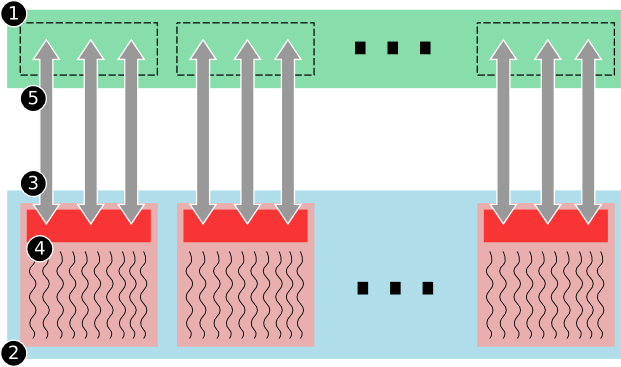
\includegraphics[width=0.6\textwidth]{img/cuda-strategy}
        \caption{GPU programming strategy}
    \end{figure}
\end{frame}

\begin{frame}[fragile]
    \frametitle{CUDA}
    \framesubtitle{Programming strategy}
    \begin{itemize}
        \item Allocating memory
        \begin{lstlisting}
            cudaMalloc((void**)&device_array, size);
        \end{lstlisting}
        \item Copying memory from Host to Device
        \begin{lstlisting}
            cudaMemcpy(device_array, host_array, size, cudaMemcpyHostToDevice);
        \end{lstlisting}
        \item Copying memory from Device to Host.
        \begin{lstlisting}
            cudaMemcpy(host_array, device_array, size, cudaMemcpyDeviceToHost);
        \end{lstlisting}
        \item Freeing memory
        \begin{lstlisting}
            cudaFree(device_array);
        \end{lstlisting}
    \end{itemize}
\end{frame}
